\documentclass[12pt,letterpaper]{article}
\usepackage{amsmath}
\usepackage{amsfonts}
\usepackage{color}
\usepackage{graphicx}
\usepackage{longtable}
\usepackage{rotating}
\usepackage{verbatim}
\usepackage[pdftex,bookmarksopen]{hyperref}
\hypersetup{pdfauthor={John Sibert}}
\hypersetup{pdfsubject={Stable Approximations}}

\newcommand\doublespacing{\baselineskip=1.6\normalbaselineskip}
\newcommand\singlespacing{\baselineskip=1.0\normalbaselineskip}
\renewcommand\deg[1]{$^\circ$#1}
\newcommand\uvD{$(uvD)$}
\newcommand\SD{SEAPODYM}
\newcommand\SDTE{SEAPODYM-TAGEST}
\newcommand\UK{uKfSST}
\newcommand\EK{ensemble Kalman filter}
\newcommand\ADMB{ADModel Builder}
\newcommand\SPC{Secretariat of the Pacific Community}
\newcommand\WCPO{Western Central Pacific Ocean}
\newcommand\SSAP{Skipjack Survey and Assessment Programme}
\newcommand\RTTP{Regional Tuna Tagging Programme}
\newcommand\PTTP{Pacific Tuna Tagging Programme}
\newcommand\FAD{fish aggregating device}
\newcommand\ADRM{advection-diffusion-reaction model}
\newcommand\help[1]{\color{red}{\it #1 }\normalcolor}
\newcommand\TT{{\tt tagest \& tagmove}}
\newcommand\TE{{\tt tagest}}
\newcommand\TM{{\tt tagmove}}
\newcommand\PAR{{\tt .par}}
\newcommand\Dunit{{nm$^2$mo$^{-1}$}}
\newcommand\Uunit{{nm~da$^{-1}$}}
\newcommand\widebar[1]{\overline{#1}}
\newcommand\EEZ{Exclusive Economic Zone}

\newcommand\Nm{{\color{red}N_{t-\Delta t}}}

\title{Stable Finite Difference Approximations}

%\author{
%John Sibert\thanks{sibert@hawaii.edu}\\
%Joint Institute of Marine and Atmospheric Research\\
%University of Hawai'i at Manoa\\
%Honolulu, HI  96822 U.S.A.\\[0.125in]
\author{John Sibert\\
\date{\today}
}


\begin{document}
\maketitle

\doublespacing

The purpose of this analysis is to explore stable recursive finite
difference equations for application to compartment models.
 
The logistic growth law is commonly used in many fish models and is a
useful starting point. 
The logistic is often written as its derivative:
\begin{equation*}
\frac{dN}{dt}= rN\Big(1-\frac{N}{K}\Big)% = rN - \frac{r}{K}N^2
\end{equation*}
Starting with the usual finite difference approximation
\begin{equation*}
\frac{dN}{dt}\approx \frac{N_t-N_{t-\Delta t}}{\Delta t} = {f(N)}_t,
\end{equation*}
the question becomes which time levels, $N_t$ and $\Nm$, should
be used  in ${f(N)}_t$?

There are 4 obvious possibilities:

The first possibility is to require the right hand side to depend entirely
on the previous time step:
\begin{equation*}
\frac{dN}{dt} \approx \frac{N_t-\Nm}{\Delta t} =
r\Nm\Big(1-\frac{\Nm}{K}\Big)
\end{equation*}
This approximation leads to
\begin{equation}
N_t = \Nm + \Delta t r \Nm\Big(1-\frac{\Nm}{K}\Big)
\label{eqn:explicit}
\end{equation}
which is sometimes known as ``explicit'' time stepping.

There are two possibilities where the right hand side depends on
different combinations of $N_t$ and $\Nm$ , that is ``semi-implicit''
time stepping.

\begin{equation*}
\frac{dN}{dt} \approx \frac{N_t-\Nm}{\Delta t} =
rN_t\Big(1-\frac{\Nm}{K}\Big)
\end{equation*}
so that
\begin{equation}
N_t = \frac{\Nm}{1-\Delta t r -\Delta t\frac{r}{K}\Nm}.
\label{eqn:implicit2a}
\end{equation}
Alternatively,
\begin{equation*}
\frac{dN}{dt} \approx \frac{N_t-\Nm}{\Delta t} =
r\Nm\Big(1-\frac{N_t}{K}\Big)
\end{equation*}
so that
\begin{equation}
N_t = \frac{\Nm(1+\Delta t r)}{1+\frac{\Delta tr\Nm}{K}}.
\label{eqn:implicit2b}
\end{equation}

The final possibility is to use fully  implicit time stepping where
the right hand side depends only on the current time step:
\begin{equation*}
\frac{dN}{dt} \approx \frac{N_t-\Nm}{\Delta t} =
rN_t\Big(1-\frac{N_t}{K}\Big)
\end{equation*}
This expression can be rearranged into standard quadratic form and
solved using the quadratic formula,
\begin{equation}
\frac{\Delta t r}{K}{N_t}^2 +(1-\Delta t r)N_t - \Nm = 0
\label{eqn:implicit}
\end{equation}
There are of course two roots; it turns out that one is positive and
one is negative. This equation of course be solved by completing the
square which might lead to a more instructive formula.

The following figures show the effects of $r$ and $\Delta t$ on
stability and accuracy. The open black circles represent the analytic
integral of the logistic equation as given by Quinn and Deriso (1999);
the red line is explicit time stepping,
equation~\ref{eqn:explicit}; 
the blue line is semi-implicit time stepping, equation~\ref{eqn:implicit2a};
the green line is semi-implicit time stepping, equation~\ref{eqn:implicit2b};
the orange line is fully implicit time stepping, equation~\ref{eqn:implicit};

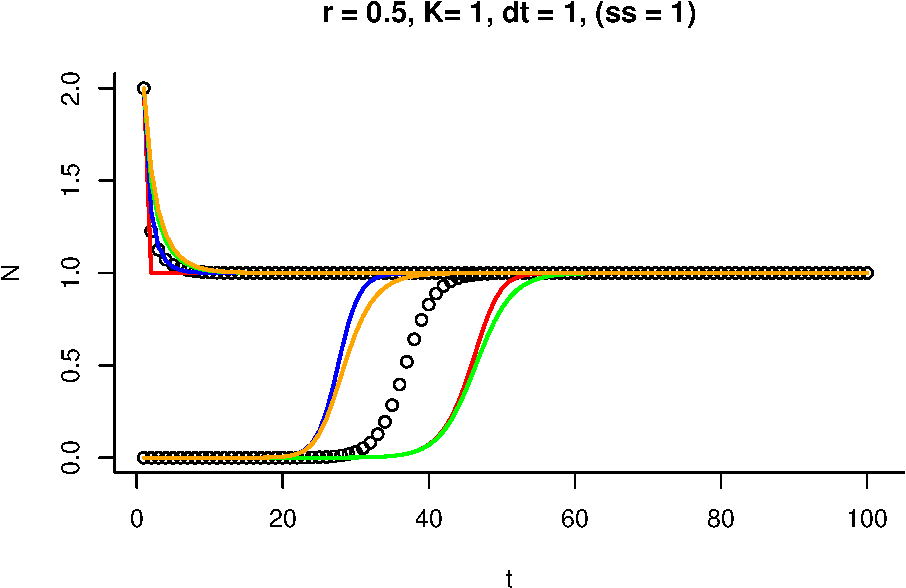
\includegraphics[width=\textwidth]{graphics/r05K1dt1ss1}
For reasonably small rate of increase $r$, all 4 approximations are stable, but
quite  inaccurate near the inflection point.

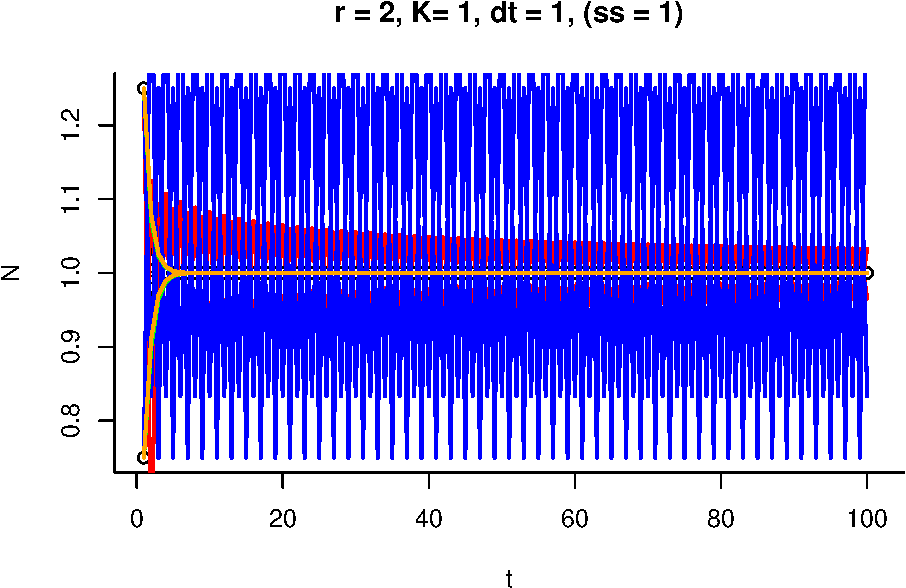
\includegraphics[width=\textwidth]{graphics/r2K1dt1ss1}
At high values of $r$, explicit approximation (\ref{eqn:explicit}) and
the semi-implicit approximation (\ref{eqn:implicit2a}) are unstable,
but the  semi-implicit approximation (\ref{eqn:implicit2b}) and fully
implicit approximation (\ref{eqn:implicit}) are stable. Again all of
the approximations are innacurate near the inflection point.

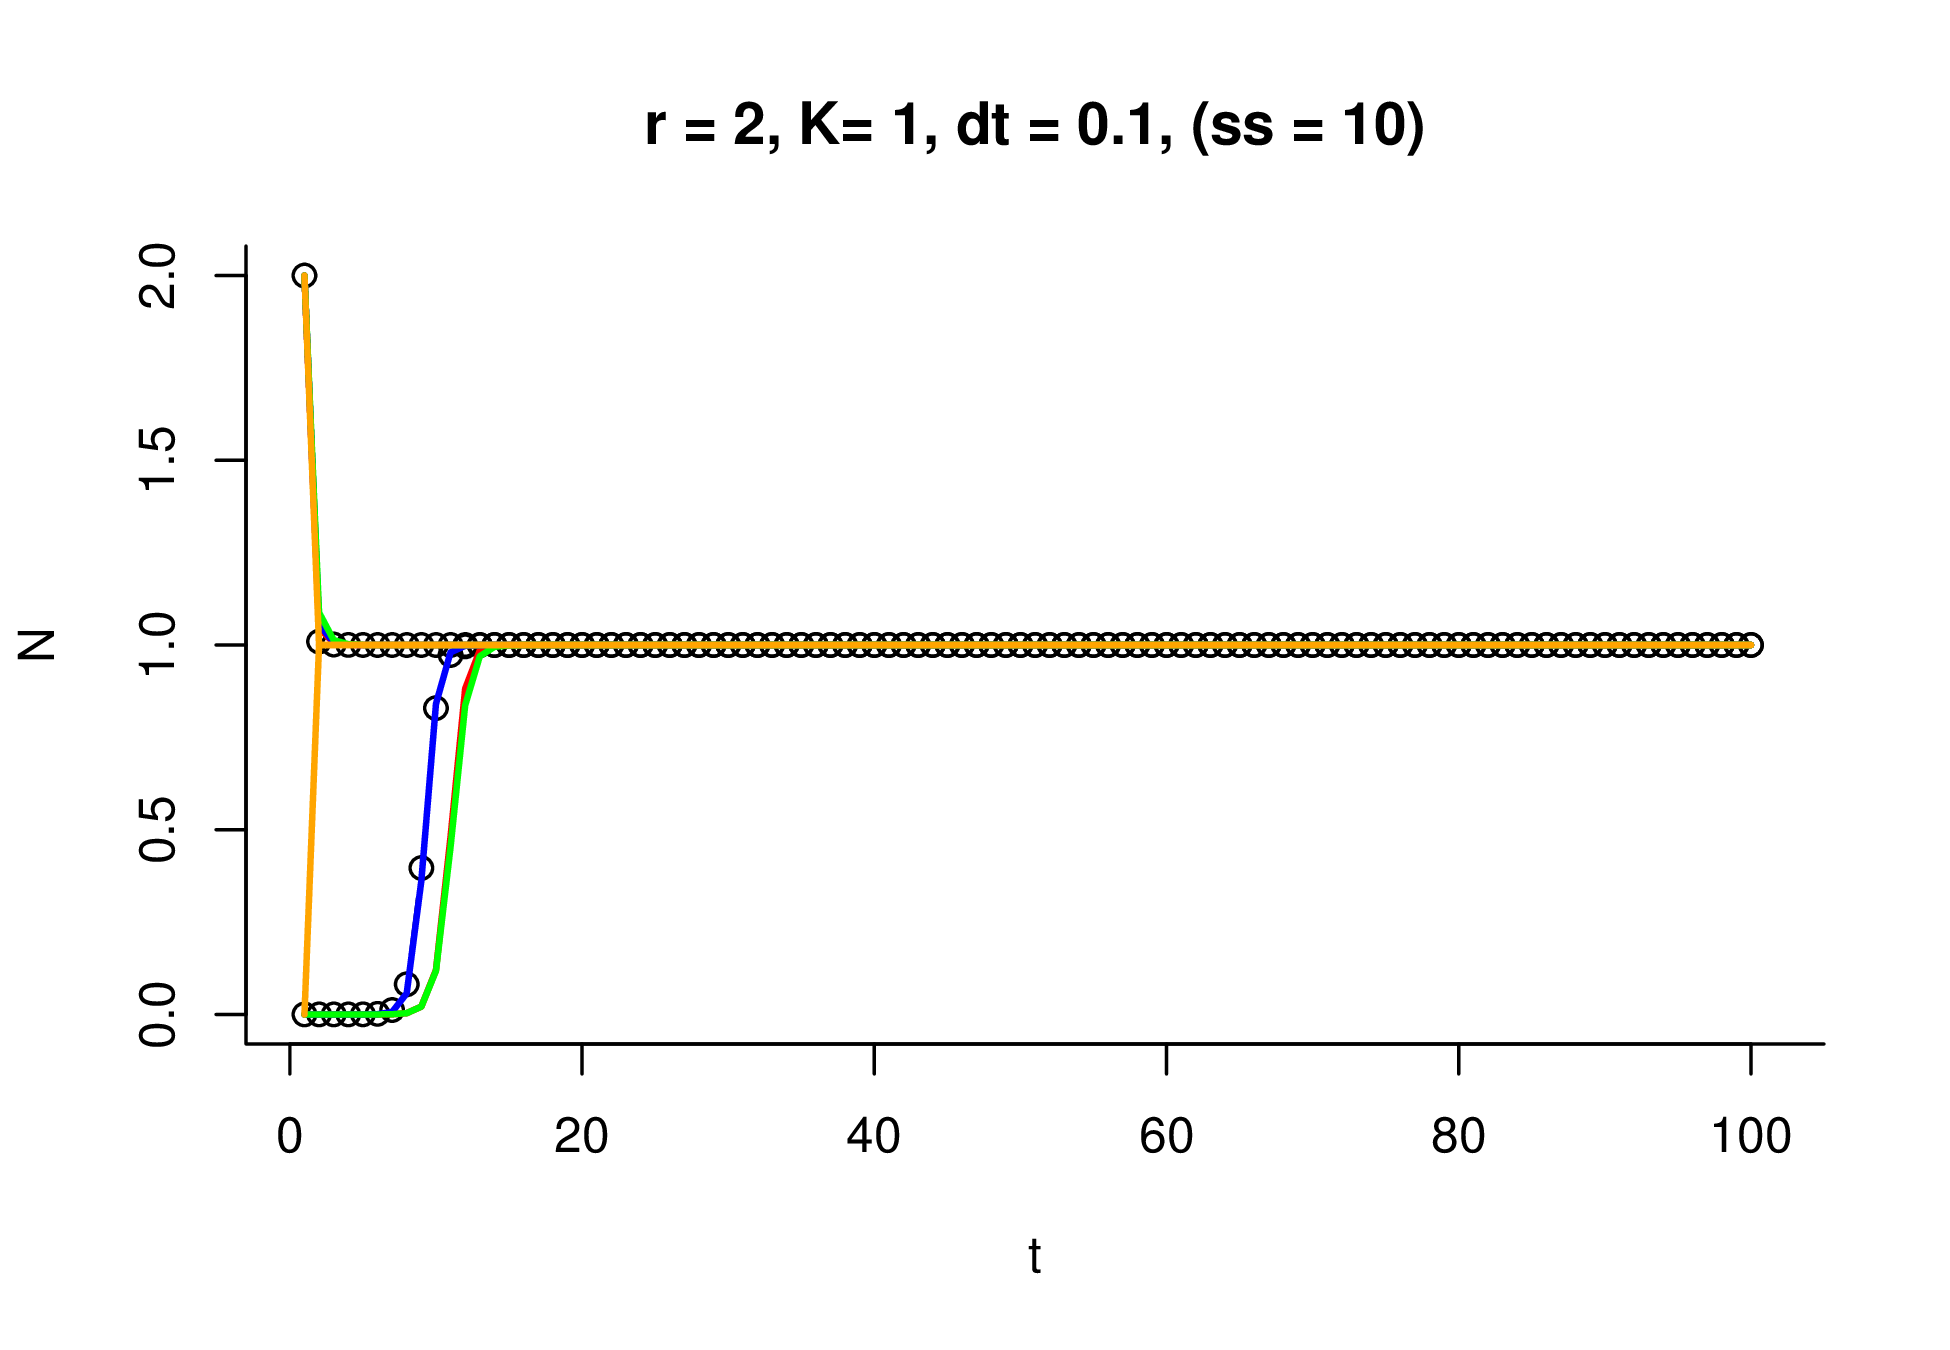
\includegraphics[width=\textwidth]{graphics/r2K1dt01ss10}
As might be expected,
decreasing the time step, $\Delta t$, at high values of $r$ increases
both stability and accuracy, especially for the semi-implicit time stepping, 
equation~\ref{eqn:implicit2a}.

\end{document}
